\documentclass[a4paper,11pt,twoside,openany]{report}
\usepackage{pslatex}
\usepackage[T1]{fontenc}
\usepackage[scaled]{helvet}
\renewcommand*\familydefault{\sfdefault}
\usepackage[top=3cm,bottom=4cm]{geometry}
\usepackage[procnames]{listings}
\usepackage{graphicx}
\usepackage{hyperref}
\usepackage{subfigure}
\usepackage{color}
\usepackage[normalem]{ulem}
\usepackage{fancyhdr}
\fancyfoot{} % clear all footer fields
\pagestyle{fancy}
\usepackage{pslatex}
\usepackage{longtable}
\usepackage{multirow}
\usepackage{lscape}
\usepackage{hyperref,url}
\usepackage{pstricks}
\usepackage{makeidx}
\usepackage{tikz}
\usetikzlibrary{chains}
\usetikzlibrary{fit}
\usetikzlibrary{positioning}
\fancyfoot[LE,RO]{\thepage}
\fancyfoot[CO,CE]{}
\fancyfoot[LO,RE]{}
%\renewcommand{\headrulewidth}{0.4pt}
\renewcommand{\footrulewidth}{0.4pt}
\setlength{\headheight}{15pt}
\newcommand{\logo}{\includegraphics[width=6cm]{/home/willijar/lib/latex/aston-logo-external-dark-blue.eps}}

\lstset{language=lisp,showspaces=false,showtabs=false,captionpos=b,xleftmargin=2em,,showstringspaces=false,keywordstyle=\color{purple},commentstyle=\color{red},basicstyle=\footnotesize,frame=leftline,procnamekeys={defgeneric,defmethod,defclass},procnamestyle=\color{blue}}
\newcommand{\cl}[1]{\lstinline{#1}}

\newcommand{\www}[2]{\href{#1}{#2}\footnote{\tt \textless{}#1\textgreater{}}}
\newcommand{\file}[1]{{\tt #1}}


\definecolor{astona}{rgb}{0 0.512 0.742}
\definecolor{astonb}{rgb}{0 0.191 0.312}
\definecolor{gray}{rgb}{0.68, 0.703, 0.668}

\makeatletter
\renewcommand\maketitle{\begin{titlepage}%
  \let\footnotesize\small
  \let\footnoterule\relax
  \let \footnote \thanks
   \begin{flushleft}
     \logo\par%
     {\sf\color{astonb}
       %
     \vfill 
     {\Huge \@title}

     {\Large \@author}
  \vfill}%
 \end{flushleft}\par%
\
\begin{center}
\vfill
\end{center}\par%
\@thanks
  \vfil\null
\end{titlepage}\thispagestyle{empty}%
\cleardoublepage
  \setcounter{footnote}{0}%
  \global\let\thanks\relax
  \global\let\maketitle\relax
  \global\let\@thanks\@empty
  \global\let\@author\@empty
%  \global\let\@date\@empty
  \global\let\@title\@empty
  \global\let\title\relax
  \global\let\author\relax
  \global\let\date\relax
  \global\let\and\relax
}
\makeatother

\renewcommand{\sectionmark}[1]{\markboth{\color{astonb}#1}{}}
\renewcommand{\subsectionmark}[1]{\markright{\color{astonb}\thesection\ #1}} 


\lstdefinestyle{ini}{
  language={[LaTeX]TeX},       % comment
  keywordstyle=\color{blue},   % comment
  basicstyle=\small\ttfamily,
  tabsize=2,
  morekeywords = {parameter},
}

\lstloadlanguages{lisp,tex,sh,[LaTeX]Tex}
\usepackage[toc,acronym]{glossaries}
\makeglossaries
\makeindex

\newglossaryentry{CL}{
        name={Common Lisp},
        description={a dialect of
    the Lisp programming language, published in ANSI standard document
    ``ANSI INCITS 226-1994 (R2004)''. It is a general-purpose,
    multi-paradigm programming language. It supports a combination of
    procedural, functional, and object-oriented programming
    paradigms. As a dynamic programming language, it facilitates
    evolutionary and incremental software development, with iterative
    compilation into efficient run-time programs.}
}

\newglossaryentry{CLOS}{
        name={Common Lisp Object System},
        description={the object oriented programming toolkit
        integrated into \gls{CL}. It supports multiple inheritance,
        mixins, multimethods, metaclasses, method combinations etc
        \ldots}
}

\newglossaryentry{MOP}{
        name={Metaobject protocol},
        description={a protocol for extending some or all of the
        internal structure of the object and class system to change the
        program semantics.}
}

\newacronym{LENS}{LENS}{Lisp Educational Network Simulator}
%\newglossaryentry{label}{name={}.description={},sort={}}
%\newacronym{label}{abbrc}{full}
\renewcommand*{\glossaryname}{List of Terms}
\renewcommand*{\abstractname}{Summary}
\renewcommand{\logo}{~\\\vfill}
\newcommand{\acr}[1]{\acrshort{#1}}

\title{LENS: Lisp Educational Network Simulator}
\author{Dr. J.A.R. Williams}

%\index{key|textbf} \index{hello!peter} \index{Peter|see{hello}}
%\nomenclature{symbol}{description}
%
%\gls{label}
\begin{document}
\maketitle

\tableofcontents

\begin{abstract}
  \acrfull{LENS} provides a generic architecture for modelling systems
  that may be represented by entities exchanging discrete messages
  over time (such as communication systems). It is designed to support
  a modular system model design (enabling model component reuse) and a
  clear separation between the model implementation and the simulated
  experiments that are being carried out in it. Models are implemented
  in \gls{CL}. Simulation experiments are specified using text
  configuration files and the results are produced in text data files
  which may then be analysed by further tools.

  This document is a manual for implementing and using models in
  \acr{LENS}.
\end{abstract}

\chapter{Introduction}
% Position
Simulations of networks can provide a useful educational tool both for
supporting traditional modular courses and for enabling students to
carry out more open ended project work. In terms of research ultralow
power wireless are an interesting engineering problem as they operate
under significant resource constraints and the protocols and
techniques that are needed are therefore very application dependant.
Simulations provide an efficient way of investigating those challenges
and potential solutions. A simulation framework that can support both
these tasks would enable students to carry out research work in
wireless sensor networks as part of their projects. 

% Problem
There are many discrete time event network simulators available. Those
which are most widely used (such as NS2 and it's derivatives) are
popular because they have been around a long time and a very large
number of network models have been written for them. The range of
models available has outgrown the original framework design and this
gives rise to many workarounds and the introduction of substantial
unnecessary complexity. This growth of baroque complexity makes it
very difficult to fully understand the details of the models or to
modify or customise them. As the models continue to grow this is
becoming harder and harder. While there have been attempts to
re-factor some of these large simulator frameworks they have met with
limited success - partly because one of the goals is to try to
maintain some sort of compatibility with the legacy of complex models.

An alternative is to design a new simulator framework based
on experience of the limitations of the previous designs which have
led to the growth in their complexity. One such framework is OMNET++
which is a simulator framework written in C++ which addresses the design
issues. The disadvantage is that it does have the wide range of network
models available as the more long standing simulators.

Traditionally simulation models are typically made up of a fixed
compiled component written in C or C++ for efficiency and a run time
interpreted component to allow customisation without having to
recompile for every model change. The run time component is either in
a dynamic extension language (such as Tcl for NS2) or a custom
language (NED for OMNET++). This simulation models are typically
spread across at least two files in two different programming
languages.  Aspects which have been fixed in the compiled model cannot
be changed at run time. It is not always transparent which aspects of
the model should be fixed and which should be configurable at model
implementation time, nor is it obvious in complex models where to find
different aspects of the implementation.

From experience I have found that students take too long to have
sufficiently in depth understanding of the Baroque mature simulators
to write new models withing the 6 month time frame allowed for Masters
projects. They are suitable for projects involving running currently
available models but not if the project is to evaluate some new model.
Additionally, when looking for a network simulator to carry out more
complete systematic evaluation of wireless sensor networks I found
that none of the already existing network simulators had
implementations of all the protocols of interest. No matter which
simulator I chose I would need to port across implementations of
protocols.

On this basis a new simulator framework \acr{LENS} has been
designed. Many aspects of the architecture are based on the excellent
design of OMNET++ however it was written entirely in
\gls{CL}. \gls{CL} provides a dynamic compiled environment with full
introspection capabilities during run time. It is an extensible
language which is especially good for domain specific customisation.
There is therefore no need to use or design a separate interpreted
language for the dynamic aspect. This simplifies the design -
typically a single protocol will be fully described in a single file
containing a class definition describing its state variables and
configurable parameters as well as its implementation.  Full use has
been made of the \gls{CLOS} to provide modularity in the design and
the associated \gls{MOP} has been used to handle cross cutting
concerns in the design.  It was considered that the initial investment
in designing the simulation framework would pay off when having to
port protocols across to it and when designing new protocols.

\chapter{Overview}

\begin{figure}
\begin{minipage}[b]{0.7\textwidth}
\begin{lstlisting}
(defclass communications(compound-module)
  ()
  (:gates
   (application :inout)
   (channel :inout))
  (:submodules
   (routing routing)
   (mac mac)
   (radio radio))
  (:connections
   (<=> application (routing application))
   (<=> (routing mac) (mac routing))
   (<=> (mac radio) (radio mac))
   (<= (radio receive) channel))
  (:metaclass compound-module-class)
  (:documentation "A Communications module"))
\end{lstlisting}
\end{minipage} \hspace{1cm}
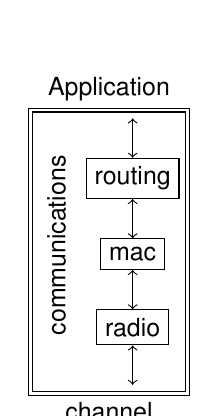
\begin{tikzpicture}[node distance=5mm,every node/.style=draw,every
  join/.style=<->,start chain=going below]
\coordinate[on chain] (application) {};
\node[on chain,join] (routing) {routing};
\node [draw=none,above left=0.2 of routing,rotate=90] (label) {communications};
\node[on chain,join] {mac};
\node[on chain,join] {radio};
\coordinate[on chain,join] (channel) {};
\node[double distance=1pt,fit=(application) (label) (routing) (channel),label=above:Application,label=below:channel] (compound) {};
\end{tikzpicture}

\caption{Compound module example with three submodules}
\label{fig:compound}
\end{figure}

\acrfull{LENS} is a discrete time event simulator. It is suitable for
simulating systems which can be represented as a set of entities
exchanging discrete messages\index{message} over time. It supports a
hierarchical design methodology where complex entities (called
compound modules\index{compound module}) are broken down into smaller
networks of components etc until we get to \index{simple module@simple
  modules} which contain the specific implementation details of the
system being modelled. The modules (whether simple or compound)
interact by send and received messages through named
gates\index{gate}. Connections between gates are represented using
channels\index{channel} which may include delays and modify the
messages (for example adding in message loss or errors).  The system
models are described and implemented using the \acrfull{CL}
programming language. Figure~\ref{fig:compound} shows an example of a
compound communications model with the \acr{CL} on the left and a
graphical representation on the right.  The system component types are
defined as classes using \acrfull{CLOS} - part of this definition is
the set of configurable parameters for the model which will be read
from a configuration file when it is being run.

Simulations are used to run a series of experiments which
varying system parameters and to collect a measurements
of the system performance for each experiment. \acr{LENS} provides
separation of the system model from the specification of the
experiments being performed. It is not necessary to change the
model to carry out different experiments. Experiments are described in
configuration files which specify what parameters to use and what
measurements are to be recorded. A single configuration file may
describe many different named experiments and may also specify a
series of experiments with varying parameters. 

The model implementation modules are instrumented by
signalling\index{signal} useful events or value changes. These signals
may be handled by the simulator to collect statistics and provide
performance evaluation reports. They might also be used to update
various views of the running simulation (for example a graphical
display).  No such graphical display is currently implemented.

The framework is generic and many different models may be
represented using it. It is recommended that a package be created for
each model which uses the \cl{:lens} package (as well as \cl{:cl}
\cl{:cl-user})) and that all declarations
for that model are made in it's package. This will prevent namespace
collisions between models. Users should then be in a particular model package
when running it. When reading parameters the \cl{:lens}  namespace is
used by default so symbols which may be read from external files will
need to be specified either with an explicit package name or be
exported into the \cl{:lens} package. Parameter names however are
parsed as strings as they are addressed by their position in the model
hierarchy and so the package in which they are declared is ignored.

% • Should be self contained as many people will only read this section!
% Briefly state:
% – The purpose of the report
% – Context overview of the background
% – Methods summary only
% – Main findings summary only
% – Main conclusions
% – Main recommendations
% • Use plain English, avoid acronyms and abbreviations.
% • Do NOT refer to figures, appendices, tables in the report.
% • Keep it short (less than 5% of the word count is a good guide).
% • This should always be written LAST and written as a separate piece of work
% NOT cut and pasted from the main report! There are three models that are
% widely used for structuring summaries:
% 1. 4Ps Position; Problem; Possibilities; Proposal
% Position beforehand, problem that you investigated, possible solutions
% and which of these you propose and why.
% 2. Problem; Cause; Solution
% Problem investigated, what is causing it and how to solve it.
% 3. Problem; Action; Result
% The original problem, what you have done about it and how it is now.


% Introduction States the objectives of the report and comments on the way the topic of
% the report is to be treated. Leads straight into the report itself. To set the scene
% and give the background and purpose to the report. It will include:
% • Background; reason for doing the work.

% • Purpose of the investigation/research.

% • Dates.
% • Methods/procedures used to get the results.

\chapter{Network Description}

Simulations are represented as a heirarchical network of
modules interconnected using channels. Every simulation must have one
top level network module which will specify submodules and their
interconnections. These submodules may be compound modules which can
contain further submodules or simple modules which contain
implementations. All module types are declared as \acr{CLOS} classes
inheriting from \lstinline{network}, \lstinline{compound-module} and
\lstinline{module} base classes as appropriate. In addition module classes
must declare a metaclass - \lstinline{compound-module-class} for
networks and compound modules and \lstinline{module-class} for simple
modules. These meta-classes allow for the declaration of parameter
slots (where the value may be initialised from the configuration
file), gates, submodules and connections in the class definition.
When a simulation is run the network type is read from the parameter
file and created. This will then create the submodules and so on until
the whole network is created.

\section{Modules}
\subsection{Network Modules}

\begin{lstlisting}[caption={An example of a simple network},label=lst:tictoc1]
(defclass TicToc1(network)
  ()                   ;; No parameters declared
  (:submodules         ;; submodule declaration
   (tic Txc1)
   (toc Txc1))
  (:connections        ;; interconnection declaration
   (=> (delay-channel :delay 0.1d0) (tic out) (toc in))
   (=> (delay-channel :delay 0.1d0) (toc out) (tic in)))
  (:metaclass compound-module-class)) ;; metaclass required
\end{lstlisting}

A network topology is described using the declaration of a new class
of type network as illustrated in listing~\ref{lst:tictoc1}. This
network is called \cl{TicToc1}. It has no slots or parameters
specified. The \cl{:submodules} class option specifies a list of two
node submodules named \cl{tic} and \cl{toc} each of must be of type
\cl{Txc1} (which we will define later). The \cl{:connections} class
option specifies connections between the gates of these submodules - in this case
there are two connections - one from the out gate of each module to
the in gate of the other module each using a channel with a delay of
0.1\,sec.

Declarations are placed in lisp files and loaded as usual
into your lisp environment. For every simulation the user will need to
specify the network name in the configuration
file.

\begin{lstlisting}[style=ini]
[General]
network=TicToc1
\end{lstlisting}

\subsection{Simple Modules}
Simple modules are the basic building blocks defining the network
behaviour. In the example above we declared two submodules each of
type \cl{Txc1} which could be declared as simple modules. A minimal
declaration is given in listing~\ref{lst:txc1}.

\begin{lstlisting}[caption={A simple module},label={lst:txc1}]
(defclass Txc1(module)
  ()
  (:gates       ;; gate declarations
   (in :input)
   (out :output))
  (:metaclass module-class)) ;; module-class metaclass required for simple modules
\end{lstlisting}

In this declaration we have defined a module which has two gates, one
input gate which can receive messages named \cl{in} and one output
gate which can send messages named \cl{out}. These named gates were
used when specifying the connections for the \cl{TicToc} network in
listing~\ref{lst:tictoc1}.

In addition to declaring the simple model class we need to define an
implementation. We do this by writing methods with the required
behaviour. In this case we want the modules to resend a message to
their output gate when they receive it on their input
gate. Additionally to get the process started we need one of the
modules to send a message on startup.

\begin{lstlisting}[caption={Txc1 Behavioural implementation},label={lst:txc1-impl}]
(defmethod initialize list ((module Txc1) &optional (stage 0))
  (when (eql (name module) 'tic)
    (send module (make-instance 'message :name 'TicTocMsg) 'out))
  t)

(defmethod handle-message((module Txc1) msg)
  (send module msg 'out))
\end{lstlisting}

After the simulator has constructed the network entities from the
definitions and configuration file the \cl{initialize} generic
function is called recursively depth first on the network hierarchy.
This takes the module an initialisation stage number as
arguments. Simple Modules define their initialisation here and return
true if their initialisation is finished. Multiple stage
initialisation is enabled. This may be necessary where there is a
cross dependence in initialisation between modules. In this case the
\cl{initialize} function will be called with increasing stage number
until it returns true i.e. if a module requires multiple stage
initialisation it should return nil until it has reached its last
stage when it should return true. In this simple example we only want
one module to start the message sending process so we check it is
named \cl{tic} and if so send a new message to the \cl{out} gate.

When a message is received by a module the \cl{handle-message} method is
called with the module and message arguments. Every simple module will
want to specialise this method to implement their behaviour. In this
example it is specialised on the \cl{Txc1} class and it immediately
calls \cl{send} to send the message to the out gate of the module.

\subsection{Compound Modules}
The above network nodes were very simple and could be implemented as
simple modules. In general however nodes will involve complex
behaviour and we will want to break their implementation down into
simpler components. A compound module can be used in this
case. Figure~\ref{fig:compound} shows an example of such a module. It
has the list of submodules and connections (as per the network
modules) as well as a list of external gates which can also be
connected to submodule gates.

Generally all of the behavioural implementation is defined in simple
modules however it is possible to add to or override some of the
default behaviour in compound modules. An example of this is were the
network of submodules and interconnections may be parameterised and
therefore a method may be added to add in the necessary network
behaviour creation before module initialisation. \footnote{This is a
  substantial difference from OMNET were all behaviour had to be in
  simple modules and a common pattern was to have to create simple
  modules that would then modify the connectivity in their parent
  compound modules}

\subsection{Gates}
Gates are the named input and output ports of both simple or compound
modules. They are given symbolic names,  and may be declared either as
\cl{:input}, \cl{:output} or \cl{:inout} (which creates both an input
and output gate of the same name. Additionally a numerical second
argument may be used to declare an array of gates. This may be 0
indicating that it the array may be extended during module
initialisation or may be the name of a module slot specifying the
size. The basic addressing
format for gates is \cl{(name [index] [direction])} or \cl{name}
which. The generic function
\begin{lstlisting}
(defgeneric gate(entity address &key index &allow-other-keys))
\end{lstlisting}
where address may be a list as above will return the gate named gate
for a module. The \cl{:index} keyword argument '++ may be used to
indicate that a new gate should be created on the addressed gate
array. If the direction is obvious from the context (e.g. it must be
\cl{:output} when sending a message) then it may be left off the
address.


\subsection{Channels}
Channels are the final component types which are used to create a
simulation. \acr{LENS} provides two inbuilt channel types. The
\cl{ideal-channel} which is the default and has zero
propagation and transmission delay and is always enabled. The
\cl{delay -channel} has a propagation delay specified using a
\cl{:delay} argument and may be disabled. In addition the
\cl{transmission-channel} base class is provided for more complex
behaviour - taking account of transmission time, packet loss etc. Most
derived channels will be based on this class and must specialise the
\cl{process-message} generic function to provide the required
functionality.

\begin{lstlisting}
(defgeneric process-message(channel message time))
\end{lstlisting}

The method should model the transmission of the given message starting
at the given time, and return the propagation delay, transmission
duration, and discard flag in a \cl{channel-result} object. The
transmission duration and bit error modeling only applies to instances
of \cl{packet} and should be skipped for non-packet messages. The
method does not need to set the duration of the packet; this is done
by the simulation kernel. However, the method should set the \cl{bit-error-p}
on the packet if error modeling results in bit errors. If the
discard flag is set in the result object, it means that the message
object should be deleted by the simulation kernel; this facility can
be used to model that the message gets lost in the channel.

The method does not need to throw error on overlapping transmissions,
or if the packet's duration field is already set; these checks are
done by the simulation kernel before \cl{process-message} is called.

In addition they may wish to implement \cl{nominal-datarate} and
\cl{calculate-duration} methods. See the file {\tt channel.lisp} for further
information on this interface.

\subsection{Parameters}

All modules and channels can be configured using named
parameters. In \acr{LENS} parameters are defined as slots in
the class definition with \cl{:parameter} argument set to true. If the
slot is not initialised by slot argument during object creation the
object will try and read a value from the configuration file. If no
value is defined in the configuration file then the default
initialisation form is evaluated and used.\footnote{Another significant
  difference from OMNET++ where the parameters were declared in the
  ned files and had to be explicitely read in the C++ implementation
  code to configure the modules.}

\begin{lstlisting}[label={lst:Txc4},caption={Compound module with a parameter}]
(defclass Txc4(Txc1)
  ((send-msg-on-init
    :parameter t :initarg :send-msg-on-init :initform nil :type boolean
    :reader send-msg-on-init
    :documentation "Whether module should send message on initialization"))
  (:metaclass module-class))
\end{lstlisting}

An example in listing~\ref{lst:Txc4}. The \cl{send-msg-on-init}
instance slot is declared as a parameter. If the initialisation
argument \cl{:send-msg-on-init} is specified during creation of a
\cl{Txc4} (either in code or in the module specification in a compound
module) then its value will be used. Otherwise the simulation
configuration will be checked for a value. Finally if neither of these
are specified the \cl{:initform} value will be used as the default. 

When declaring parameter slots you should specify a
format to be used to parse the configuration string into an internal
type. By default this is derived from the declared slot \cl{:type}
however the slot \cl{:format} may be used to customise this parsing
for example to allow for additional error checking. This argument
takes any format type specification understood by the
\cl{data-format-validation} library and new format types may be added
as per that library. If no format or type are declared the parameter
will be read in as a string.

\chapter{Messages and Packets}

Message objects in \acr{LENS} are used to represent events, packets,
commands, jobs, customers and other types of entities depending on the
model domain. They may be sent through gates and channels between
modules or may be send directly to a module. The base \cl{message}
class records the creation time, transmission time, arrival time and
the source and destination entites.

The generic function
\begin{lstlisting}
(defgeneric send(from-module message gateid &key delay))
\end{lstlisting}
Provides the basic mechanism for a module to send a message out
through one of its named gates. The gate can be an actual gate object
or it's specifier.

The simulator will call \cl{handle-message} with the module and
message when at the message arrival time.

Packet objects are messaged used to represent network packets.

\begin{lstlisting}
(defclass packet(message)
  ((encapsulated-packet
    :type packet :initarg :encapsulated-packet
    :documentation "Higher level encapsulated protocol packet.")
   (duration :accessor duration :type time-type :initform 0.0d0
             :documentation "Duration of last transmission")
   (control-info
    :accessor control-info :initarg :control-info
    :documentation "Additional data to be passed with packet between
    protocol layers")
   (reception-start-p :accessor reception-start-p
    :type boolean :initform nil :initarg :deliver-on-reception-start
    :documentation "Identify whether this packet represents the start
or the end of the reception after the packet travelled through a
channel with a data rate. This flag is controlled by the
deliver-on-reception-start flag of the receiving gate.")
   (bit-error-p
    :initform nil :reader bit-error-p
    :documentation "The result of error modelling after the packet is
sent through a channel that has a nonzero packet error rate (PER) or
bit error rate (BER). It is up to the receiver to examine this flag
after having received the packet, and to act upon it."))
   (:documentation "Representation of network packets"))
\end{lstlisting}

All message and packet types must override the \cl{duplicate} method
to provide proper duplication semantics (i.e. must explicitely copy
slots from an originating packet to a duplicate one. The
\cl{encapsulate} and \cl{decapsulate} methods are used to embed and
access higher level encapsulated packets. Duplication does results in
the originating and duplicate packets sharing the same encapsulated
packet - however decapsulating returns a duplicate of the encapsulated
packet ensuring appropriate copy semantics are maintained
efficiently through this interface.

The \cl{control-info} field in packets may be used to pass additional
information with packets as they are passed between protocol layers -
for example command information to a lower layer as the packet is
passed down or additional information associated with packet reception
as the packet is passed up a protocol stack.

\chapter{Signals and Instrumentation}

For a simulation to be useful it must collect useful information on
the model operation. Separating our the generation of the information
from the collecting and reporting of it allows for the maximum
flexibility and generality. The \acr{LENS} this is achieved with the use
of named signals which may be emitted with useful information in the
model implementation code and which can then be collected and analysed
by listeners attached to the various modules in the simulation.

The function \lstinline{(defun register-signal(symbol \&optional
  documentation))} is normally called as a top level form to register a
particular named signal with the symbol. Adding documentation is
recommended so that other implements may reuse it if they have similar
semantics. Registering commonly used signals ensures that their
handling will be optimised.

In the model implementation the \lstinline{(defgeneric emit(entity
  signal &optional value))} method is called to broadcast a
signal. This may optionally take an argument (for example a count)
associated with that signal. Listeners registered to receive this
signal in the broadcasting module or above it in the hierarchy will
all receive the signal in via the \lstinline{(defgeneric
  receive-signal(listener signal source-component value))} method.
If the generation of the broadcast signal is expensive the \lstinline{
(defun may-have-listeners(entity signal-id))} function may be called to
check whether it is necessary first.

Modules call the \lstinline{(defgeneric subscribe(entity signal
  listener))} and \lstinline{(defgeneric unsubscribe(entity signal
  listener))} functions to register or unregister a listener object
for a particular signal on a particular module. A listener may be
registered to more than one signal or module and can use the
source-component, signal and value arguments to differentiate the
source as required).

As an example an application module might register signals for packet
transmission and reception at the top level in the source file.

\begin{lstlisting}
(register-signal
 'packet-receive
 "Emitted when application receives a packet.")

(register-signal
 'packet-send
 "Emitted when application sends a packet.")
\end{lstlisting}

In the relevant code implementation for transmission and reception it may call
\cl{(emit application 'packet-send packet)} or \cl{(emit application
  'packet-receive packet)} respectively to inform the relevant listeners of
these events. These send the actual packet as a value. Listeners
should not modify the packet but may read values from them.

\subsection{Statistics}

Network instrumentation is performed by registering listeners which
can receive signals and perform the relevant analysis. These are
registered as part of a module class declaration as statistic
properties of that module e.g.

\begin{lstlisting}
(defclass application(wsn-module)
  ( 
    ;; parameter declarations
   )
  (:gates
    ;; gate declarations
  }
  (:properties
   :statistic (latency
               :source (latency packet-receive)
               :title "application latency"
               :default ((histogram :min 0)))
   :statistic (packet-receive :title "application packets received"
                              :default (count))
   :statistic (packet-receive-per-node
               :title "packets received per node"
               :source (source (control-info packet-receive))
               :default (indexed-count))
   :statistic (packet-send :title "application packets sent"
                           :default (count)))
  (:metaclass module-class)
  (:documentation "Application connects to sensors for measurements
  and to communication module for sending/receiving data."))
\end{lstlisting}

This example declares four different statistics associated using the
\cl{packet-send} and {packet-receive} signals. Each statistics is
given a name and title (used in reports), a source declaration (a
function which when applied to the signal value will return a number)
and a list of default and optional statistics to be performed on the
source value. These statistics are registered listener classes which 
will collect their received values and produce either scalar or
vector outputs from the simulation for analysis. See the
\file{statistics.lisp} and \file{statistics-impl.lisp} core files for
more information. Whether a particular statistic is active or not is
controlled in the simulation configuration file - those declared as
default are active unless turned off and those declare optional are
not active unless turned on in the configuration file. The
framework allows for the implementation and declaration of new
statistic listener types if required. 

\chapter{Configuring Simulations and Experiments}

\appendix

\bibliographystyle{plainnat}
\bibliography{references}

\printindex

\printglossaries

\end{document}
